\begin{savequote}[75mm]
	``Self-driving cars are the natural extension of active safety and obviously something we thing we should do."
	\qauthor{Elon Musk}
\end{savequote}

\chapter{Introduction}
%\addcontentsline{toc}{chapter}{Introduction}
In robotic research, the problem of navigation is among the most important. Basically, all autonomous mobile robots need some kind of navigation abilities to perform, localization, motion planning and guidance \cite{Skoda:Thesis:2016}. In the present context, we focus on navigation as a process of planning a path of a mobile robot from its current position to a desired goal location, following the planned path, and avoiding any discovered obstacles along the way. The desired paths have to fulfill several conditions to ensure safety and feasibility of the navigation. Moreover, the paths can be also defined in terms of specifications; for example, short or smooth paths are usually more desirable than long and curved ones in every dynamic environments. Beyond the path planning, the navigation problem also involves reacting to changes of the environment model. Robots are required to move towards the target in a short time and avoid either static or dynamic obstacles observed by their sensors, which involves efficient path planning and valid obstacle avoidance. Research and development of Unmanned Ground Vehicles has been dominated by DARPA (Defense Advanced Research Projects Agency) and NASA (National Aeronautics and Space Administration). The DARPA initiative started with the development of the first mobile robot, Shakey, and also includes the Autonomous Land Vehicle and the DARPA Demo I1 Program. NASA sponsors the development of unmanned vehicles for planetary surface exploration, from the Jet Propulsion Laboratory Mars Rover to the most recent Mars Pathfinder. Recent UGV design and development has been enhanced to build UGVs capable of operating in Intelligent Vehicle Highway Systems \cite{Bai2015}. Over the last decades, the development of Advanced Driver Assistance Systems has become a critical endeavor to attain different objectives: safety enhancement, mobility improvement, energy optimization and comfort \cite{Gruyer2017}. Much of the argument used in this discussion is based on the road mortality we see today. According to data from the World Health Organization, in 2013 there were about 1.25 million road deaths worldwide, and this number is expected to increase in the next decade \cite{world2015global}. Algorithms for autonomous navigation are increasingly robust and reliable and are starting to handle complex situations and decision problems. According to Katrakazas \cite{Katrakazas2015}, local navigation is responsible for guiding the vehicle, that is, for the planning of the direction and speed to be taken, in a space close to the current position based on information exclusively obtained by the sensors on board. The guiding must be planned in such a way as to guarantee the displacement, from the current state to the objective, without collisions. The algorithms we have developed at the LAR, follow a new and different approach for an advanced control strategy for autonomous navigation. The idea is that these methods do not replace the algorithms developed previously but are a valid alternative, so that depending on the situation, the vehicle can choose the best strategy to overcome obstacles or solve problems that can occur on the road that need a decision in real time.  Simulation results demonstrate and verify the feasibility and the usefulness of methods considering different scenarios.

In this introductory chapter, the ATLAS project is presented in more detail in section \ref{sec:ATLAS}, while examples of autonomous navigation projects are discussed later (section \ref{sec:autonomous_examples}). The context of the problem and the proposed solution of this thesis are carried out in section \ref{sec:context} while the organization of the document is discussed in section \ref{sec:outline}.
\section{ATLAS Project}\label{sec:ATLAS}
The ATLAS project was created in 2003 by the Group for Automation and Robotics from the Department of Mechanical Engineering at the University of Aveiro \cite{vsantos2010}. The objective of this project is to study and develop advanced sensors and active systems to promote the autonomous control of cars and other platforms. The first projects in the autonomous driving area focused on small scale models in controlled environments for participation in the National Robotics Festival (FNR) and in many other competitions winning some awards for the best performance (subsection \ref{sec:ATLASplatform}). The success and experience gained with these models allowed the evolution of the project for full-scale vehicles, where ATLASCAR (subsection \ref{sec:ATLASCAR}) in 2010 and ATLASCAR2 (subsection \ref{sec:ATLASCAR2}) in 2016 have been developed.

\subsection{ATLAS platforms}\label{sec:ATLASplatform}	
The first developed robot (Figure \ref{fig:modelosatlas1}) was based on an aluminum and wood structure. In this prototype only one camera was installed that pointed to a mirror to allow the complete visualization of the road in which the robot circulated. The traction movement was assured by a mechanical differential coupled to the rear wheels and the steering movement was given by a single front wheel. In order to create a model more similar to an ordinary car, the ATLAS group developed the ATLAS 2000 (Figure \ref{fig:modelosatlas2}) in scale (1:4), with which it managed to win the first autonomous driving competition of the FNR in 2006. After several improvements made in ATLAS 2000, in 2008 a new platform, ATLAS MV (Figure \ref{fig:modelosatlas3}) was created. This robot was designed on a smaller scale (1:5), with the intention of being lighter and faster. On board were installed a new steering system, hydraulic braking and an active perception unit. This robot allowed the conquest of new victories in the autonomus driving competitions.
\begin{figure}[!h]
	\centering
		\begin{minipage}[t]{0.32\textwidth}
			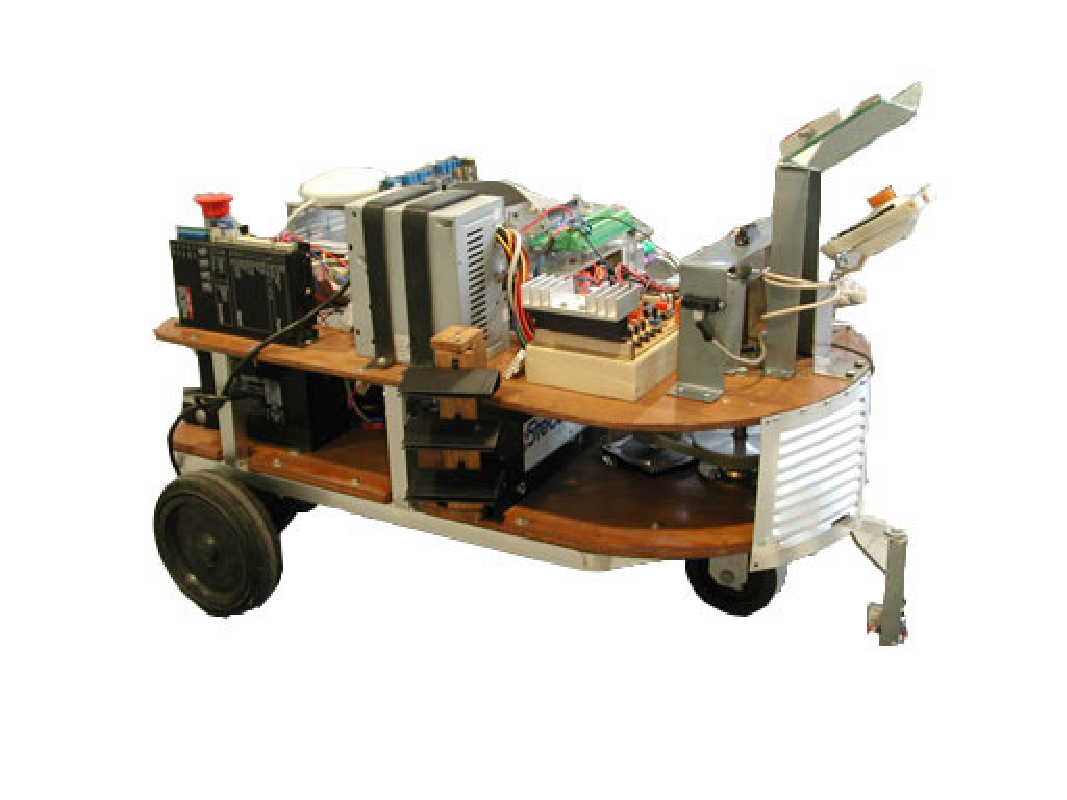
\includegraphics[width=\textwidth]{./figure/modelosatlas1.pdf}
			\subcaption{First ATLAS prototype.}
			\label{fig:modelosatlas1}
		\end{minipage}
		\begin{minipage}[t]{0.32\textwidth}
			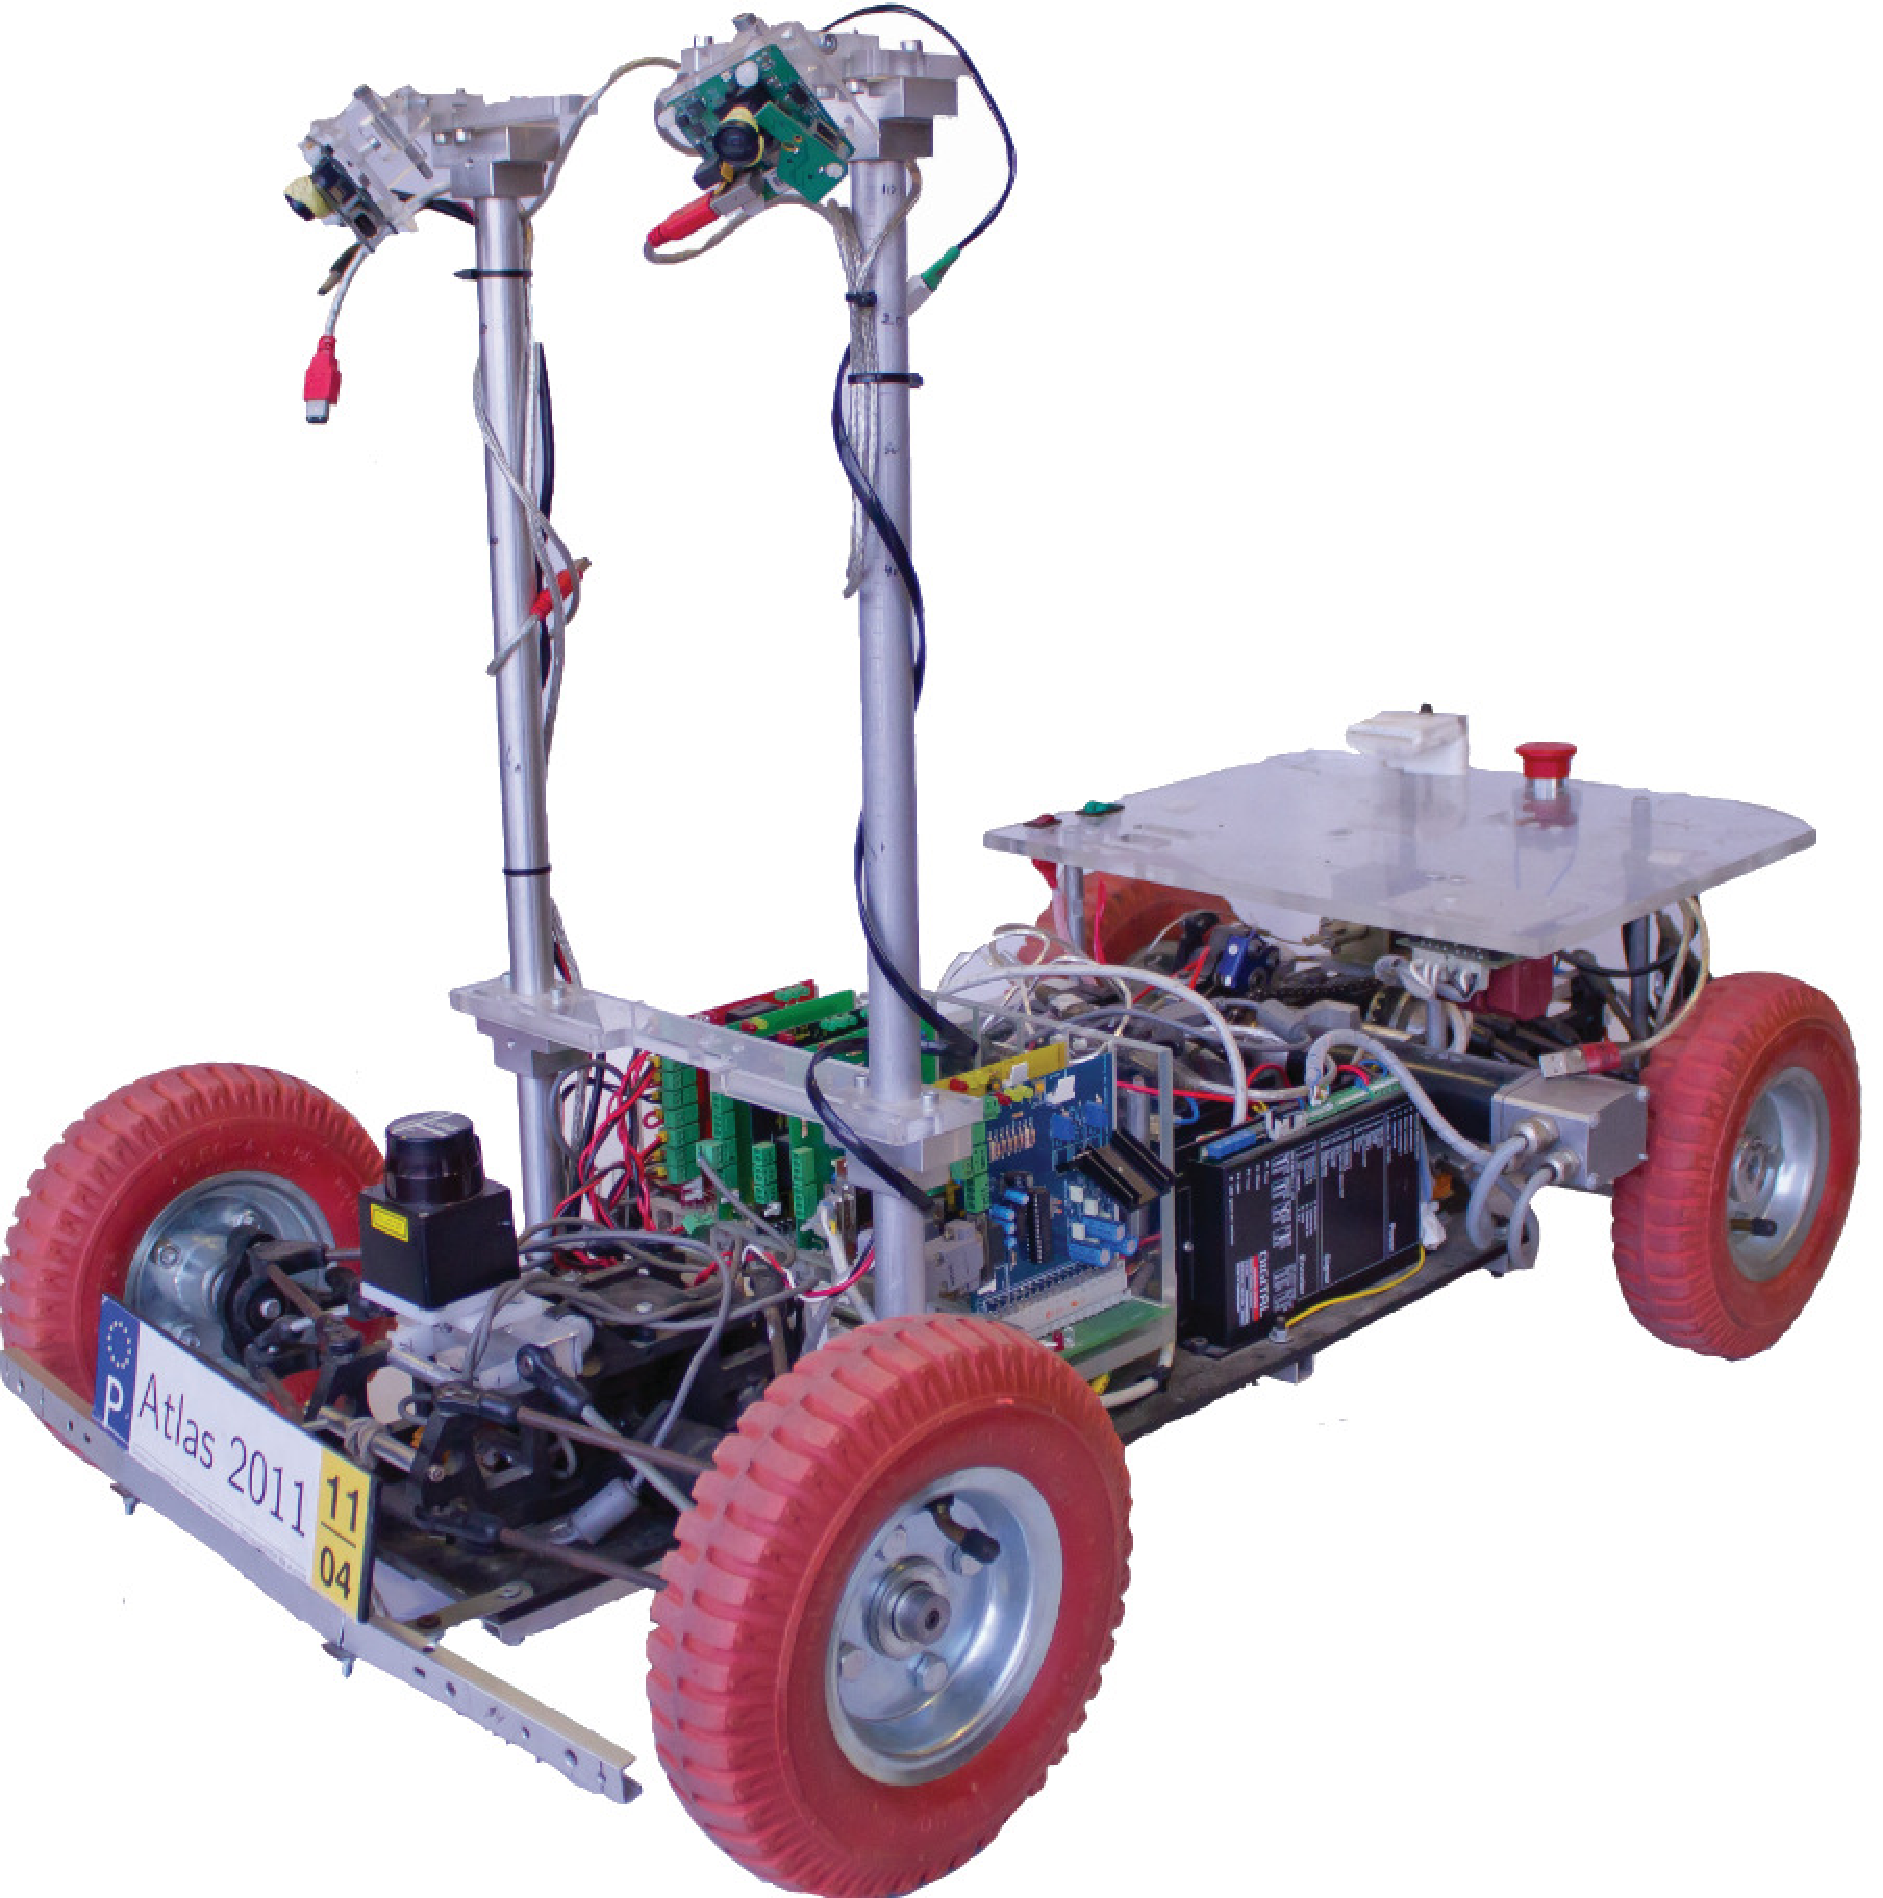
\includegraphics[width=\textwidth]{./figure/modelosatlas2.pdf}
			\subcaption{ATLAS 2000.}
			\label{fig:modelosatlas2}
		\end{minipage}
		\begin{minipage}[t]{0.32\textwidth}
			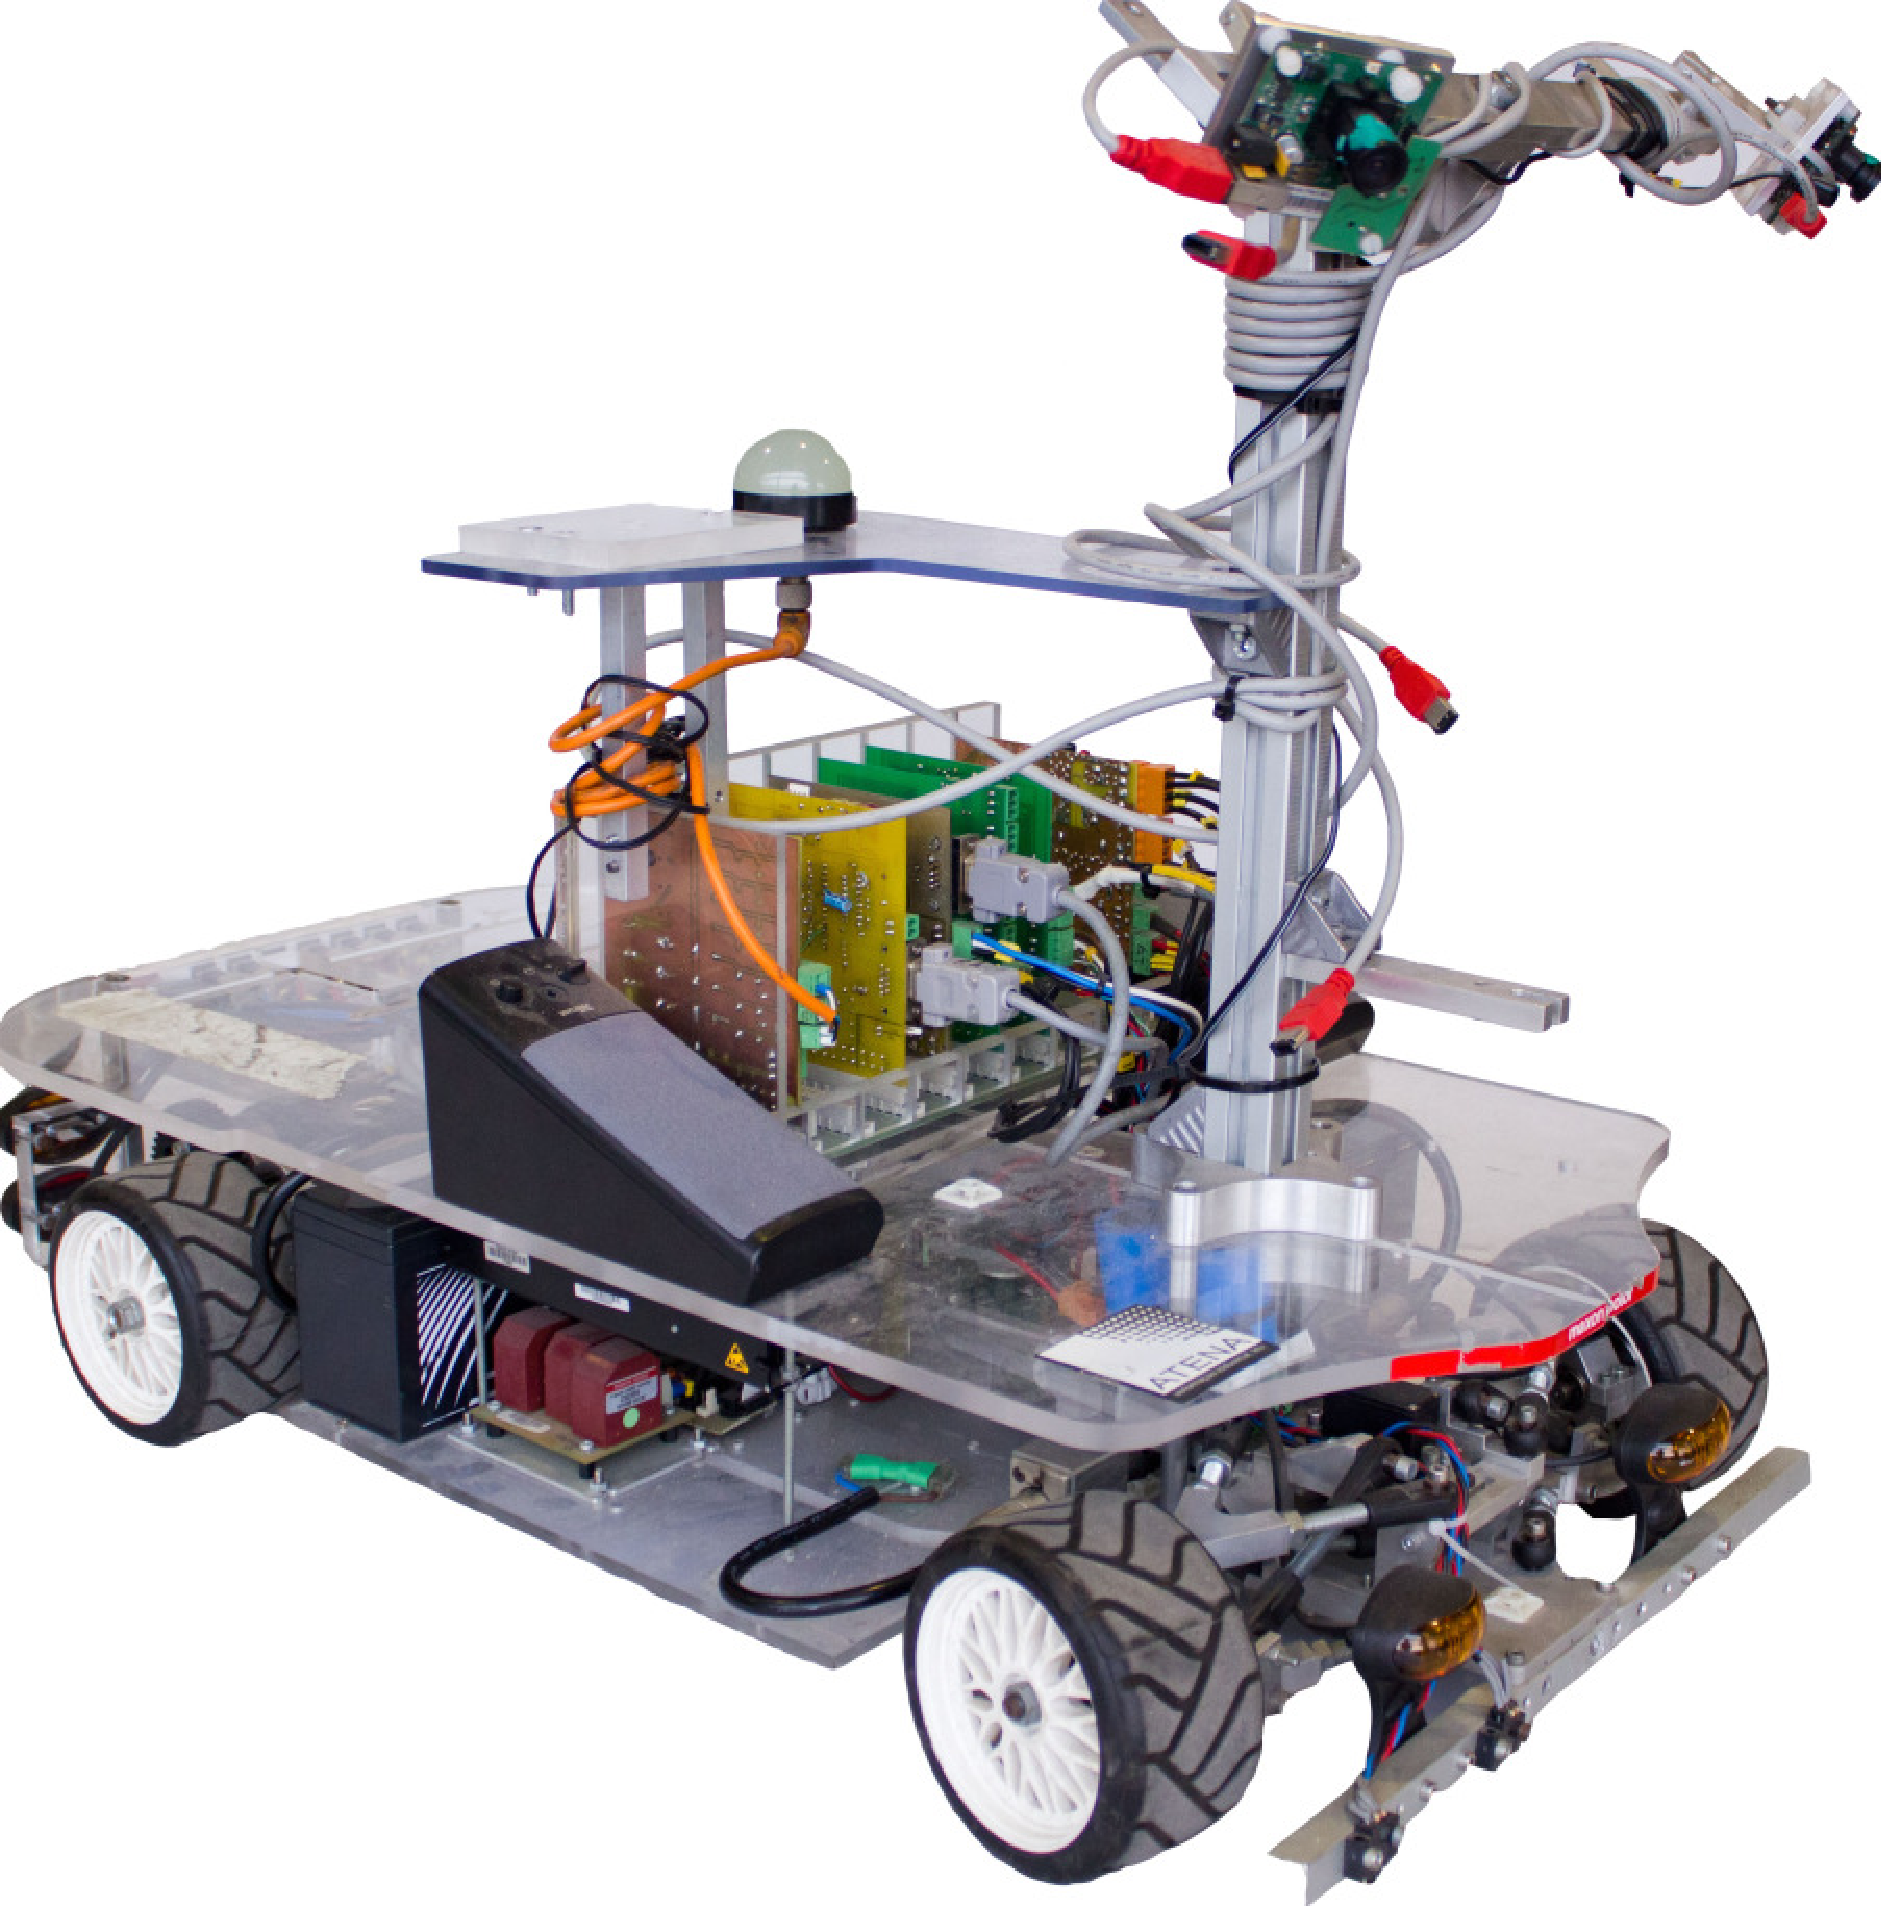
\includegraphics[width=\textwidth]{./figure/modelosatlas3.pdf}
			\subcaption{ATLAS MV.}
			\label{fig:modelosatlas3}
		\end{minipage}
		\caption{Some of the ATLAS project small scale platforms (adapted from \cite{Pereira2012}).}
		\label{fig:modelosatlas}
\end{figure}

\subsection{ATLASCAR}\label{sec:ATLASCAR}
Driven by the positive results achieved with scale models and years of navigation experience in controlled environments, in 2010 the Group of Automation and Robotics decided to invest in a large-scale project, ATLASCAR (Figure \ref{fig:atlascar1}). The vehicle used for this project was a Ford Escort Station Wagon of 1998 powered by a gasoline internal combustion engine, in which several sensors, processing units and actuators were installed. On-board sensors processed data collected from the vehicle and its surroundings, with different LIDARs for obstacle detection and environmental reconstruction, pedestrian detection cameras and a Global Navigation Satellite System (GNSS) for location and route planning. After passing through the processing units, these data were sent to the actuators that allowed the movement and execution of the maneuvers in a completely autonomous way on the part of the vehicle. To power all the equipment, a Uninterruptible Power Supply (UPS) was used, loaded from an auxiliary alternator. During this project, many works were developed in the Laboratory for Automation and Robotics, many of which produced master thesis. For example, in 2014 Cabral de Azevedo \cite{Azevedo2014} developed a module to detect pedestrians using sensory fusion of LIDAR and vision data while in 2016 Vieira da Silva \cite{Silva2016} created a multisensory calibration module that was exported to subsequent projects.
\begin{figure}[!h]
	\centering
	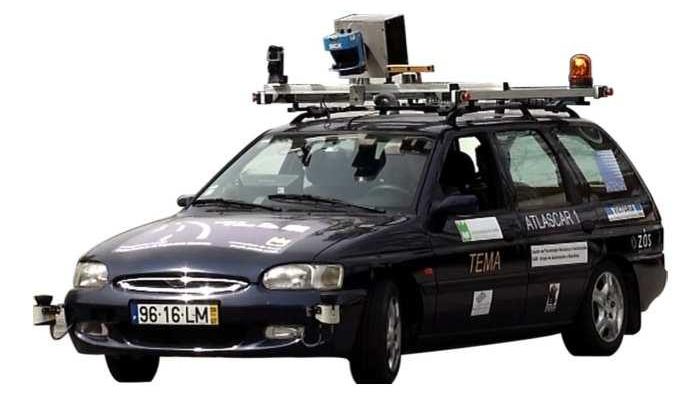
\includegraphics[width=0.9\textwidth]{./figure/atlascar1.jpg}
	\caption{The car used in ATLASCAR, based on Ford Escort Station Wagon of 1998 (adapted from \cite{Pereira2012}).}
	\label{fig:atlascar1}
\end{figure}

\subsection{ATLASCAR2}\label{sec:ATLASCAR2}
Given the different limits, to continue the project, in 2016, a new vehicle was acquired: ATLASCAR2 (Figure \ref{fig:atlascar2}). This time it was chosen as a platform
an electric car, a Mitsubishi iMiEV, with an autonomy range of \SI{100}{km}. The fact that the vehicle is electric allows to use the energy stored in the batteries, making it easier to power the sensors installed. In fact, despite the short time of existence, 3 LIDARs, a camera, inclinometry sensors and a GNSS unit are already installed on the ATLASCAR2. Many of these sensors were transferred from ATLASCAR to this project during the work of Madureira Correia \cite{Madureira2017} in 2017, where a module for detecting free space around the car was also developed while in 2018 Ricardo Silva \cite{Ricardo:Thesis:2018} created a local navigation module for driver assistance in the immediate decision making, identifing a solution based on a multiple hypothesis approach.
\begin{figure}[!h]
	\centering
	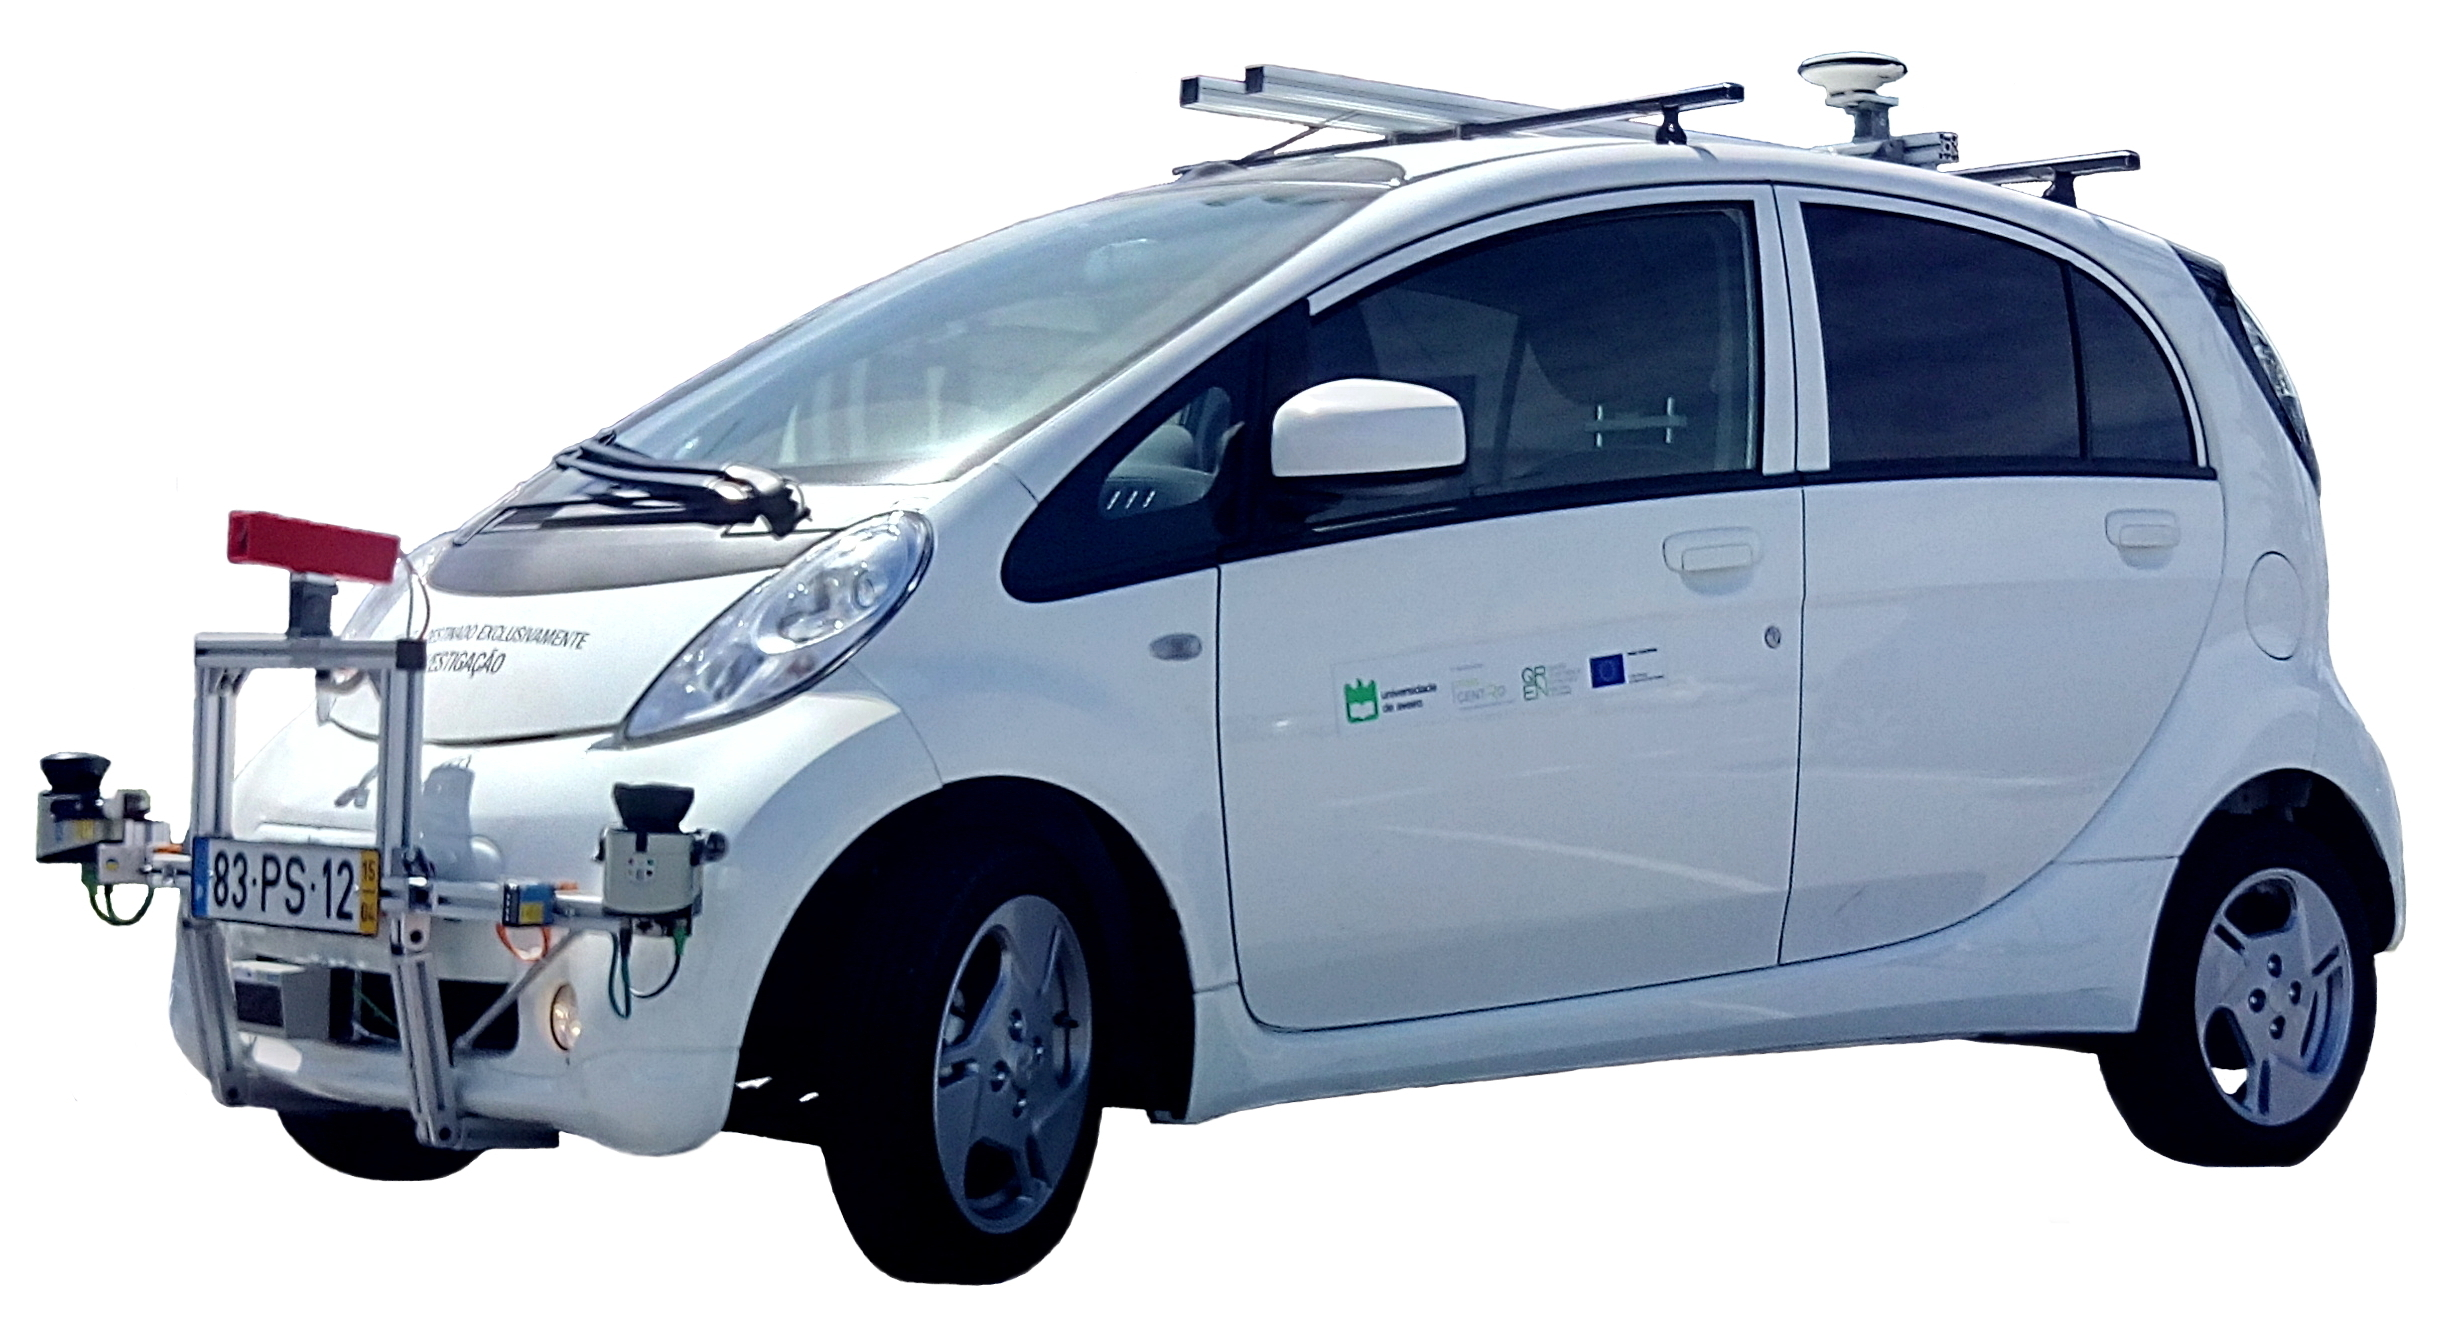
\includegraphics[width=0.85\textwidth]{./figure/atlascar2.jpg}
	\caption{The vehicle used in ATLASCAR2, based on an electric car, a Mitsubishi iMiEV of 2015 (adapted from \cite{Ricardo:Thesis:2018}).}
	\label{fig:atlascar2}
\end{figure}

\section{Autonomous Cars}\label{sec:autonomous_examples}
The legal definition of autonomous vehicle in the District of Columbia code \cite{DColumbia} is:
\begin{quotation}
	\itshape ''Autonomous vehicle'' means a vehicle capable of navigating District roadways and interpreting traffic-control devices without a driver actively operating any of the vehicle's control systems. The term ''autonomous vehicle'' excludes a motor vehicle enabled with active safety systems or driver-assistance systems, including systems to provide electronic blind-spot assistance, crash avoidance, emergency braking, parking assistance, adaptive cruise control (ACC), lane-keep assistance (LKA), lane-departure warning, or traffic-jam and queuing assistance, unless the system alone or in combination with other systems enables the vehicle on which the technology is installed to drive without active control or monitoring by a human operator. 
\end{quotation}

The modern automobile companies keep coming up with newer autonomous features in their recent models. Technological advancements seen every day in areas like information technology, communication, data analysis and storage etc. is not exclusive to these areas alone. The realm of autonomous cars is also progressing at a rapid rate these days \cite{Bimbraw2015}. Google's development of self-driving technology began in January 2009. The initial objective of the project was to develop a car able to navigate on highways with minimal human intervention. In December 2016, the unit was renamed Waymo; this name derived from its mission, "a new way forward in mobility". Waymo moved to further test its cars on public roads after becoming its own subsidiary.
\begin{figure}[!h]
	\centering
	\begin{minipage}[t]{0.45\textwidth}
		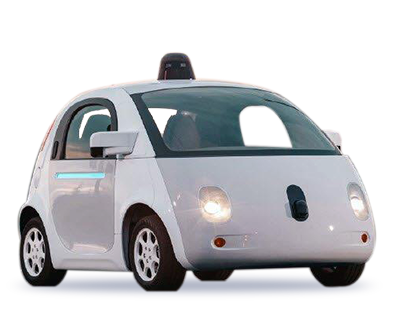
\includegraphics[width=\textwidth]{./figure/veiculos0.png}
		\subcaption{Google's Firefly self-driving prototype in 2015 (adapted from \cite{waymoh}).}
		\label{fig:veiculos0}
	\end{minipage}
	\begin{minipage}[t]{0.45\textwidth}
		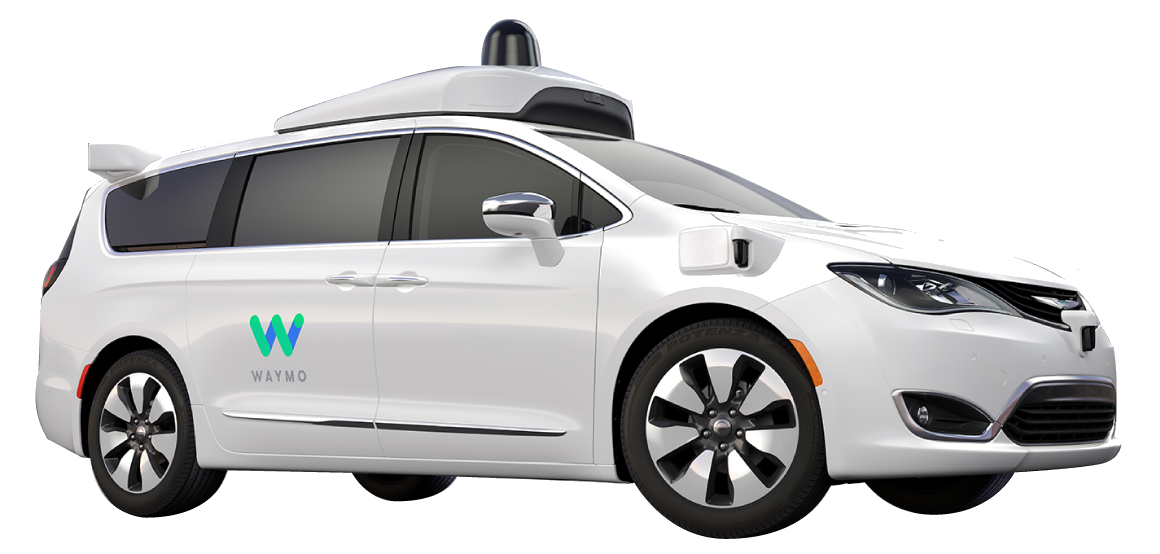
\includegraphics[width=\textwidth]{./figure/veiculos1.png}
		\subcaption{Waymo Chrysler Pacifica Hybrid self-driving prototype in 2017 (adapted from \cite{waymoh}).}
		\label{fig:veiculos1}
	\end{minipage}
	\caption{Some of the Waymo/Google prototypes tested across multiple locations in the Unided States in recent years.}
	\label{fig:waymo}
\end{figure}

Waymo uses LIDAR which sends out millions of laser beams per second to build up a detailed picture of the world all 360 degrees around it. It also uses radar to detect how far away objects are and their speed and high-resolution cameras detect visual information like whether a traffic signal is red or green. It then combines all that data to understand the world around it and predict what those things might do next. It can do that for things up to three football fields away. Based on all this information, Waymo's software determines the exact trajectory, speed, lane and steering maneuvers needed to progress along this route safely \cite{waymoh} \cite{waymot}.

With the advances in autonomous technology, VIAC or VisLab Intercontinental Autonomous Challenge was one of the major competitions which led to improvements in the testing and analysis of autonomous vehicles and robotics. It was a 13,000 kilometers trip, nearly three months from Parma, Italy to Shanghai, China from July 20, 2010 to October 28, 2010. It involved four autonomous vehicles with negligible human intervention and high level of autonomy \cite{Broggi2010}. One of VisLab's advanced autonomous car, BRAiVE (Figure \ref{fig:veiculos4}), drove in downtown Parma on July 12th, 2013. It successfully navigated narrow rural roads, crosswalks, traffic lights, pedestrian areas, roundabouts and artificial hazards. It was a pioneer in the field of vehicular robotics, since it was totally autonomous \cite{Broggi2013}.
\begin{figure}[!h]
	\centering
	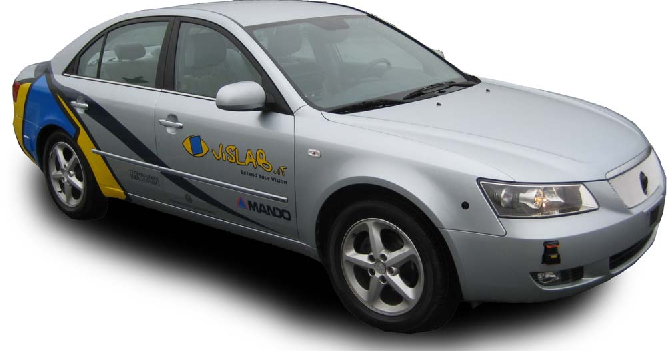
\includegraphics[width=0.65\textwidth]{./figure/veiculos4.png}
	\caption{BRAiVE prototype developted by VisLab, based on a Hyundai Sonata (adapted from \cite{Broggi2013}).}
	\label{fig:veiculos4}
\end{figure}

Another example of autonomous system is Navya, a robotically driven electric shuttle which operates at a maximum speed of 25 kilometers per hour. Made by Induct Technology, France, it can accommodate 15 passengers. It uses four LIDAR units and stereoscopic optical cameras, and it does not
require any road modifications. Its LIDAR unit and
optical cameras help in generating a real-time three dimensional map of the surroundings. It is being successfully tested at various universities across Switzerland, England and Singapore \cite{Zhang2014}.

\begin{figure}[!h]
	\centering
	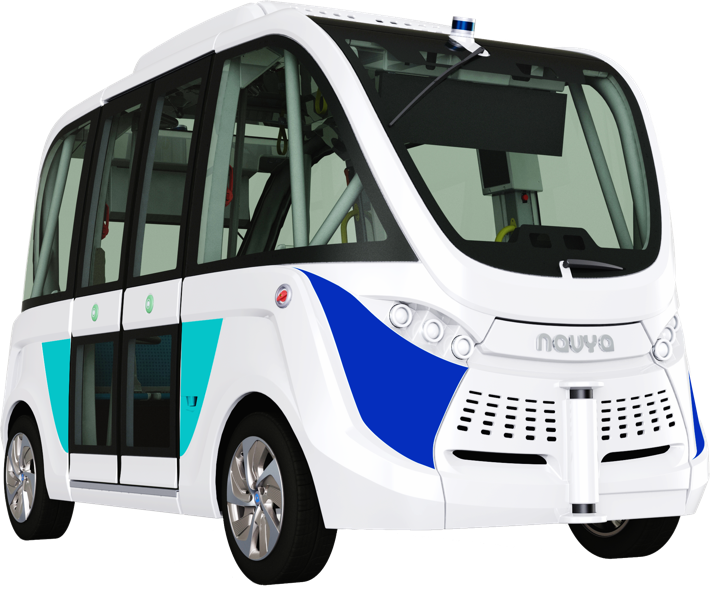
\includegraphics[width=0.6\textwidth]{./figure/veiculos5.png}
	\caption{Navya Shuttle developted in 2016 by Navya Group in France.}
	\label{fig:veiculos5}
\end{figure}

\section{Context of the Problem and Proposed Approach}\label{sec:context}
Dynamic environments pose several added difficulties to the motion planning problem. The dynamics of the ATLASCAR2 must be taken into account, and there are limitations due to the sensors range and uncertainty in measurements, that must be reflected on the motion plan. Besides it, a motion plan must incorporate time restrictions, meaning the vehicle will require a certain amount of time to accomplish a task. For example, when crossing a road, the ATLASCAR2 must do it fast enough to avoid incoming cars. The proposed algorithms were studied for the ATLASCAR2 project in which the group for Robotics and Automation at the University of Aveiro has setup and adapted a common commercial electric vehicle to provide a versatile  framework  to  develop  studies  and  research \cite{vsantos2010} \cite{vsantos2019}. The fact that the vehicle is electric allows to use the energy stored in the batteries, making it easier to power the sensors installed. In fact, the ATLACAR2 is equipped with sensors, such as lidar, that measure the distance to obstacles in front and around the vehicle. The obstacles can be static, such as a large pothole, or moving, such as a moving vehicle on the same or a nearby lane. The most common maneuver from the driver is to temporarily move to another lane, drive past the obstacle, and move back to the original lane afterward. In this case, we want to design an obstacle avoidance system that moves the ATLASCAR2 around  moving obstacles in the lane using throttle and steering angle. This system uses an adaptive Model Predictive Controller that updates both the predictive model and the mixed input/output constraints at each control interval. Moreover we want to develop a lane-keeping assist system for the vehicle: it has a sensor, such as camera or laser, that measures the lateral deviation and relative yaw angle between the centerline of a lane and the ATLASCAR2; it also measures the current lane curvature and its derivative. Depending on the curve length that the sensor can view, the curvature in front of the vehicle can be calculated from the current curvature and its derivative. This system keeps the autonomous car travelling along the centerline of the lanes on the road by adjusting the front steering angle. The goal for lane keeping control is to drive both lateral deviation and relative yaw angle close to zero.

\section{Thesis Outline}\label{sec:outline}

In this section, we outline the thesis organization: 

Chapter 1 is used to introduce the thesis focus areas of autonomous vehicle technology. In particular the ATLAS project and examples of autonomous navigation projects are presented. Moreover the context of the problem and the objectives to be achieved are carried out.

Chapter 2 focuses on some of the more theoretical aspects of this dissertation with a brief introduction to path planning, a literature review related to local navigation algorithms with a special section centred on MPC control strategy for obstacle avoidance and tracking.

In Chapter 3, the theory of Model Predictive Control is discussed in detail to highlight working principle and its characteristics (tuning parameters, stability and robustness). In particular for this work we used an advanced control strategy based on this paradigm called Adaptive MPC that uses a fixed model structure, but allows the model parameters to evolve with the time.

Chapter 4 is used to present the Obstacle Avoidance method that we have developted. First we introduced the case-study model, then we designed the decision making alghorithm and the controller. Finally we verified the control strategy in different scenarios.

Chapter 5 focuses on the Lane Following alghoritm based on Adaptive Model Predictive Control. We considered a different model in which we have applied the bicycle model of lateral vehicle dynamics and approximated the longitudinal dynamics using a first order transfer function.
Then we developed the overall control scheme considering different paths to follow.
